\documentclass[11pt,a4paper,twoside]{article}
\usepackage[includeheadfoot, left=3cm, right=2cm, top=2.5cm, bottom=2.5cm, headheight=19.3pt]{geometry}

\usepackage[polish]{babel}
\usepackage[T1]{fontenc}
\usepackage[utf8]{inputenc}
\usepackage[scaled]{helvet}
\renewcommand\familydefault{\sfdefault} 

\let\lll=\relax
\usepackage{amsmath}
\usepackage{amsfonts}
\usepackage{amssymb}
\usepackage{bm}

\usepackage{url}
\usepackage{pdfpages}
\usepackage[bookmarks, pagebackref]{hyperref}
\usepackage[none]{hyphenat}
\usepackage{graphicx}
\usepackage{color}
\usepackage{array}
\usepackage{etoolbox, fancyhdr, xcolor}
\usepackage[hang, flushmargin]{footmisc}
\usepackage{setspace}
\usepackage{ragged2e}
\usepackage{MnSymbol}
\usepackage[nottoc]{tocbibind}
\usepackage{titlesec}
\urlstyle{rm}
\usepackage[ampersand]{easylist}
\usepackage{enumitem}
\setlist[itemize]{noitemsep, topsep=0pt, leftmargin=*, itemindent=-1cm}
\usepackage{epsfig}
\usepackage{float}
\usepackage[font={up, footnotesize}, labelfont=bf, singlelinecheck=off, format=hang]{caption}
\usepackage{caption}
\usepackage{subcaption}
\usepackage{listings}
\lstset{language=C++, rulecolor=\color{sapphire}, framerule=1.5pt} % you can change language of your code
\usepackage{colortbl}
\usepackage{tabu}
\usepackage{makecell}
\usepackage{boldline}
\setlength{\arrayrulewidth}{1pt}
\captionsetup[table]{name=Tabela}

\usepackage{lipsum} % for testing purposes

\definecolor{sapphire}{RGB}{120,150,207}
\definecolor{grafit}{RGB}{60,60,60}

% pdf output setup
\hypersetup{
	unicode,
	pdftoolbar,
	pdfmenubar,
	pdffitwindow,
	pdfstartview = {FitH},
	pdftitle = {Praca Inżynierska}, 
	pdfauthor = {Ahata Valiukevich},
	pdfnewwindow,
	colorlinks,
	linktoc = page,
	% use color sapphire or grafit
	linkcolor = sapphire,
	citecolor = sapphire,
	filecolor = sapphire,
	urlcolor = black
}


\newcommand{\itemi}[1][sapphire]{\item[\color{#1} $\filledsquare$]}
\newcommand{\itemii}[1][sapphire]{\item[\color{#1} $\square$]}
\newcommand{\itemiii}[1][sapphire]{\item[\color{#1} $\bullet$]}

\ListProperties(Hide=100, Progressive=1cm, Style=\color{sapphire}, Style**=\color{black}, Style*=$\square$ ,Style2*=$\bullet$)


\newcommand{\headrulecolor}[1]{\patchcmd{\headrule}{\hrule}{\color{#1}\hrule}{}{}}
\newcommand{\footrulecolor}[1]{\patchcmd{\footrule}{\hrule}{\color{#1}\hrule}{}{}}


\newcommand{\infostyle}[1]
{
	\fancyhf{}
	\fancyhead[LO]{\Large{\textbf{#1}}}

	\renewcommand{\headrulewidth}{1.5pt}
	\headrulecolor{sapphire}
	\justify
	\pagestyle{fancy}
}


\newcommand{\thesisstyle}
{
	\fancyhf{}
	\fancyhead[RO,LE]{\Large{\textbf{\rightmark}}}
	\fancyfoot[LE,RO]{\thepage}

	\renewcommand{\headrulewidth}{1.5pt}
	\renewcommand{\footrulewidth}{1.5pt}
	\headrulecolor{sapphire}
	\footrulecolor{sapphire}
	\justify
	\pagestyle{fancy}
}


\newcommand{\fancyfootnotetext}[2]
{
	\fancypagestyle{footnotes}
	{
    	\fancyfoot[LO,RE]{\parbox{15cm}{\footnotemark[#1]\footnotesize #2}}
	}
	\thispagestyle{footnotes}
}


\newcommand{\fancyfootnotetexts}[4]
{
	\fancypagestyle{footnotes}
	{
    	\fancyfoot[LO,RE]{\parbox{15cm}{\footnotemark[#1]\footnotesize #2 \\ \footnotemark[#3]\footnotesize #4}}
	}
	\thispagestyle{footnotes}
}


\newcommand{\fancyfootnotetextss}[6]
{
	\fancypagestyle{footnotes}
	{
    	\fancyfoot[LO,RE]{\parbox{15cm}{\footnotemark[#1]\footnotesize #2 \\ \footnotemark[#3]\footnotesize #4 \\ \footnotemark[#5]\footnotesize #6 \\}}
	}
	\thispagestyle{footnotes}
}


\titlespacing\section{0pt}{15pt}{10pt} 
\titlespacing\subsection{0pt}{15pt}{10pt} 
\titlespacing\subsubsection{0pt}{15pt}{10pt} 

\setstretch{1.15}
\setlength{\parindent}{0.5cm} 
\setlength{\parskip}{0cm} 

\frenchspacing
\sloppy

\author{} 
\title{} 
\date{}
\graphicspath{{images/}}
\begin{document}

\includepdf[pages={-}]{preamble/begining.pdf}
\tableofcontents
\thispagestyle{empty}
\thesisstyle
\newpage 

\section[Wstęp]{Wstęp}
W przeciągu ostatnich kilku lat nauka zrobiła duży postęp w kierunku rozwoju fizyki dużych energii. Osiągnięcie to składa się z wyników dużej liczby badań oraz eksperymentów prowadzonych w różnych naukowo-badawczych instytucjach. Równolegle z naukami fizycznymi rozwiajała się również branża informatyczna, a w szczególności grafika komputerowa. Obecnie jest obserwowany coraz silniejszy trend związany z rozwojem technik stereoskopowych. Przy połączeniu badań fizycznych i grafiki komputerowej powstaje możliwość dogłębnego przestudiowania zjawisk zachodzących podczas rożnych eksperymentów. 
%3D television and 3D glasses are becoming much more prevalent with the latest trends in consumer electronics and technological advances in wearable computing. In the market, there are currently many hardware options that allow us to visualize information with stereoscopic 3D technology.
% The ability to visualize data in a stereoscopic 3D environment provides a powerful and highly intuitive platform for the interactive display of data in many applications. For example, we may acquire data from the 3D scan of a model (such as in architecture, engineering, and dentistry or medicine) and would like to visualize or manipulate 3D objects in real time.

\subsection{Cele i zakres pracy}
Pierwszym celem niniejszej pracy dyplomowej jest stereoskopwa wizualizacja detektora oraz zdarzeń ciężkich ionów w eksperymencie ALICE. Kolejnym istotnym celem pracy jest połączenie wyżej wymienionych wizualizacji do jednego spójnego obrazu.

Dla realizacji celi podstawowych niezbędne jest zapoznanie się z technologią stereoskopii i aktualnie dostępnymi rozwiązaniami, przestudiowanie podstaw działania eksperymentu ALICE oraz środowiska informatycznego w CERN.

Celem pośrednim danej pracy jest zapoznanie się z możliwościami biblioteki OpenGL, a także innymi uwarunkowaniami ważymi w aspekcie projektowanej aplikacji.

\subsection{Słownik użytych terminów}
Ze względu na brak jednolitego tłumaczenia niektórych zasadniczych terminów z języka angielskiego na język polski, przedstawione jest nazewnictwo użyte w niniejszej pracy dyplomowej. Tłumaczenia były zbierane głównie w oparciu o różne słowniki oraz literaturę specjalistyczną.
\begin{itemize}
\itemi Renderować (-ruje) --- ang. rendering, tworzyć realistyczne obrazy komputerowe \cite{pwn}.
\itemi Shader (-ra, -rze; -ry, -rów) --- moduł cieniujący, nieduży program w procesorze graficznym \cite{slownik}.
\itemi Antyaliasing (-ngu, -ngiem)  --- ang. anti-aliasing, zespół technik służących usuwaniu zakłóceń powstających przy renderowaniu obrazu \cite{wprowadzeniedografiki}.
\itemi Asemblacja --- ang. assembling, montaż, zebranie, zgromadzenie prymitywu \cite{slownik}.
\itemi Teselacja --- ang. tessellation, dzielenie wygenerowanych podczas tworzenia obrazu 3D wielokątów na mniejsze \cite{slownik}.
\itemi Rasteryzacja --- ang. rasterisation, działanie polegające na jak najwierniejszym przedstawieniu płaskiej figury geometrycznej na urządzeniu rastrowym \cite{slownik}.
\itemi Track (-a, -ów) --- ślad, ścieżka poruszania się cząstki w detektorze.
\itemi Uniform (rmu, -rmie; -rmów) --- zmienna globalna do przekazywania danych z aplikacji do procesora i z procesora do modułów cieniujących \cite{slownik}.
\end{itemize}
\newpage
\section[Część analityczna]{Część analityczna}
\subsection{Stereoskopia}
Stereoskopia --- to technika służącą do tworzenia iluzji głębi obrazu, nie zapewnia ona prawdziwie trójwymiarowych widoków, ale zapewnia efekt trójwymiarowości. Każdemu oku obserwatora jest prezentowany inny widok, dlatego sceny wydają się mieć głębię.

Istnieje kilka różnych technik osiągnięcia efektu stereoskopowego. Każda technika ma własny materiał stereoskopowy, inaczej stereogram, oraz sposób przeglądania dostosowany do konkretnego celu. W dalszej części niniejszej pracy są przedstawione krótkie opisy kilku technik streoskopowych cieszących się dużą rozpoznawalnością. Niektóre z nich są odpowiednie tylko dla jednego widza, podczas gdy istnieją techniki sprawdzające się dla większej grupy odbiorców.
\subsubsection{Historia} 
Historia stereoskopii liczy już ponad 180 lat. Za odkrywcę uważa się Charlesa Wheatstone'a, który jako pierwszy zaobserwował zjawisko widzenia stereoskopowego, opisał go w artykule oraz skonstruował urządzenie potwierdzające słuszność jego teorii \cite{stereoscopehistory}.

Wheatstone wyjaśnia, że jeśli obiekt znajduje się w małej odległości od oczu, to każde oko widzi przedmiot pod nieco innym kątem, z innej perspektywy. Zaś dla obiektów na dużej odległości nie ma to znaczenia \cite{wheatstone}. Wykorzystując te obserwacje naukowiec skonstruował urządzenie, które umożliwiło przedstawienie delikatnie różniących się obrazów prawemu i lewemu oku z osobna z powstającą w efekcie iluzją trójwymiarowości obrazu.

\subsubsection{Stereogramy typu side by side}
Najprostszą metodą doświadczenia widzenia stereoskopowego jest umieszczenie dwóch oddzielnych obrazów obok siebie (ang. side by side). Perspektywa jednego z obrazów reprezentuje lewe oko, odpowiednio druga perspektywa jest dla oka prawego. Obrazy te można zazwyczaj oglądać bez użycia dodatkowych narzędzi. Jedyna różnica polega na sposobie ich oglądania. Jeśli obraz dla lewego oka znajduje się po lewej stronie, to stosuje się technikę patrzenia równolegległego, w innym przypadku obrazy mają być oglądane z użyciem techniki skrośnej. Zastosowanie niewłaściwej metody spowoduje odwrócenie efektu stereoskopowego. Może to ujawnić się w postaci zniekształconych odległości pomiędzy obiektami na obrazie lub oddalenia się dwóch obrazów.

Warto zauważyć, że oglądanie stereogramów tworzy duże obciążenie dla oczu. W celu zmniejszenia negatywnych skutków używa się stereoskopu bądź specjalnego ekranu 3D w zestawie z okularami. To w znacznej mierze redukuje przemęczenie oczu i pozwala przez dłuższy czas przyglądać się efektom widzenia stereoskopowego.
\begin{figure}[H]
		\centering
 		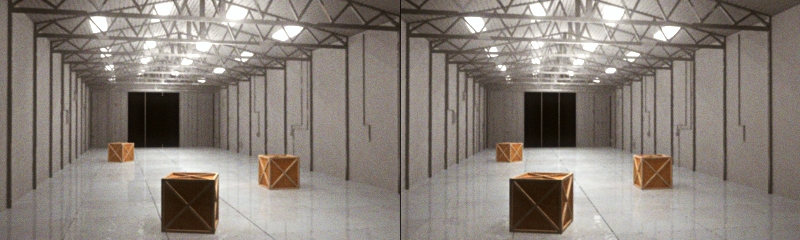
\includegraphics[width=10cm]{sbs.jpg}
 		\captionsetup{font={up, footnotesize}}
    	\caption{Stereogram \cite{sidebyside}.}
 		\label{rys1}
\end{figure}

\subsubsection{Stereogramy typu single-image} 
Stereogramy typu single-image, inaczej nazywane autostereogramy, to zbiór punktów, które wydają się tworzyć trójwymiarową scenę, gdy są skrośnie oglądane z bliska. Do osiągnięcia efektu stereoskopowego za pośrednictwem autostereogramów nie są potrzebne żadne urządzenia, aczkolwiek okulary pryzmatyczne ułatwiają przegladanie poprzeczne, a także nad- i podgląd.

Przy użyciu poprawnej techniki oglądania specjalnie stworzonego obrazu powstaje wrażenie trójwymiarowości. Czasem obrazy mogą wyglądać jak zniekształcone lub losowo umieszczone kolorowe plamy. Taki wygląd w rzeczywistości nie jest przypadkowy, ponieważ poprzez użycie powtarzalnego wzoru są ukrywane obiekty trójwymiarowe \cite{stereoscopythesis}.

\subsubsection{Stereoskopia pasywna} 
Do tworzenia iluzji obrazów trójwymiarowych są wykorzystywane specjalnie spolaryzowane okulary, które ograniczają światło docierające do każdego oka. W celu przedstawienia widoku stereoskopowego dwa obrazy są wyświetlane na tym samym ekranie z użyciem różnych filtrów polaryzacji. Istenieją 2 rodzaje filtrów: liniowe oraz kołowe.

W przypadku liniowej polaryzacji pole elektryczne światła jest skierowane pionowo bądź poziomo. Odbiorca zakłada odpowiednio dopasowane okulary, w których każda soczewka przepuszcza światło o innym kierunku polaryzacji. W ten sposób oczy obserwują różniące się obrazy. Minimalne pochylenie okularów może spowodować niezgodność polaryzacji światła a soczewek. Nieporządany efekt można wyeliminować korzystając z filtrów kołowych prawo- lub lewoskrętnych. Ruch ten pozostaje niezmienny, nawet jeśli okulary są dowolnie pochylone.

Niewątpliwą zaletą stereoskopii spolaryzowanej jest to, że wiele osób może oglądać obrazy stereoskopowe w tym samym czasie \cite{russianpage}. Wadą tego rozwiązania jest koszt specjalnego ekranu do wyświetlania obrazów. Taki ekran musi posiadać srebrną warstwę, dzięki czemu nie zniekształca się polaryzacja obrazów przy jednoczesnym wyświetlaniu.
\begin{figure}[H]
		\centering
 		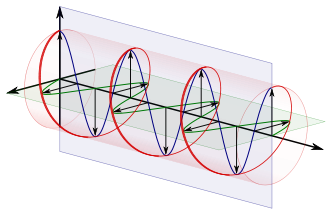
\includegraphics[width=8cm]{circular.png}
 		\captionsetup{font={up, footnotesize}}
    	\caption{Polaryzacja kołowa prawoskrętna \cite{polarization}.}
 		\label{rys3}
\end{figure}

\subsubsection{Stereoskopia aktywna} 
Możliwość oglądania obrazów stereoskopowych pojawia się dzięki ciekłokrystalicznym okularom migawkowym. Szkło, które tworzy soczewki okularów, zawiera ciekłe kryształy oraz filtr polaryzacyjny. Stosując napięcie można zmienić kolor soczewki na czarny, co bezpośrednio wiąże się z blokowaniem widoku dla jednego oka. Dzięki przykrywaniu widoku z dużą częstotliwością, każdemu oku są przedstawiane obrazy z różną perspektywą \cite{active3d}. Częstotliwość migotania okularów jest zsynchronizowana z aktualnym źródłem wyświetlania, żeby stale dostarczać prawidłowej perspektywy dla oczu. Jeśli prędkość aktualizacji soczewek w okularach nie jest wystarczająco wysoka, to może nastąpić zauważalne zniekształcenie obrazu końcowego. Przykładem takiego zniekształcenia może posłużyć część obrazu ze złą perspektywą, przeznaczona innemu oku.
\begin{figure}[H]
		\centering
 		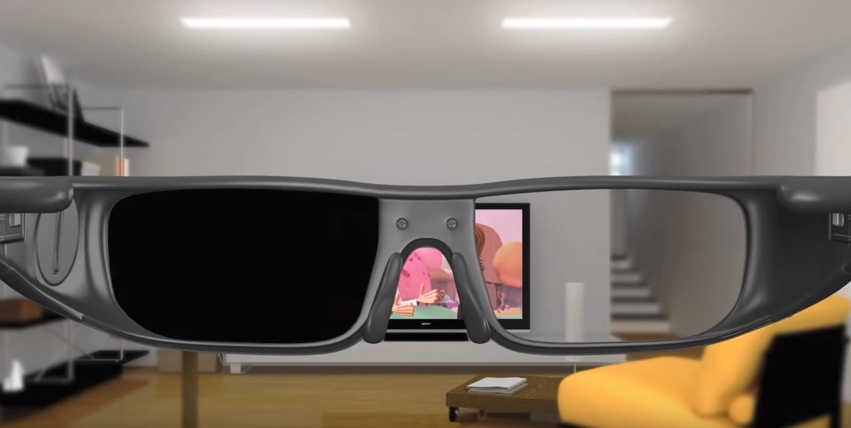
\includegraphics[width=10cm]{telewizor.png}
 		\captionsetup{font={up, footnotesize}}
    	\caption{Stereoskopia aktywna \cite{active3d}.}
 		\label{rys2}
\end{figure} 

\subsubsection{Techniki anaglifowe}
Do generowania stereogramu anaglifowego potrzebne są 2 obrazy z delikatnie różniącą się perspektywą dla każdego oka. Każdy obraz jest wykonany w podstawowych kolorach. Najbardziej popularną kombinacją jest obraz w kolorze czerwonym dla lewego oka i obraz wykonany w przy połączeniu zielonego i niebieskiego (otrzymany kolor nazywa się cyan) odpowiednio dla prawego oka. Obrazy umieszcza się jeden nad drugim. Efekt stereoskopowego widoku jest osiągany przy użyciu okularów z poprawnymi kolorowymi filtrami (podobnie jak obrazy: czerwony dla lewego oka, cyan dla prawego). Niestety przy użyciu tej techniki nigdy nie zostanie stworzony pełnokolorowy obraz, gdyż barwy widziane przez każde oko są ograniczane \cite{anaglif}. 

Istenieją także filtry o innych kolorach, zachowując główną zasadę anaglifów: przedstawienie innych obrazów każdemu oku poprzez ograniczenie pewnych barw.

\begin{figure}[H]
		\centering
 		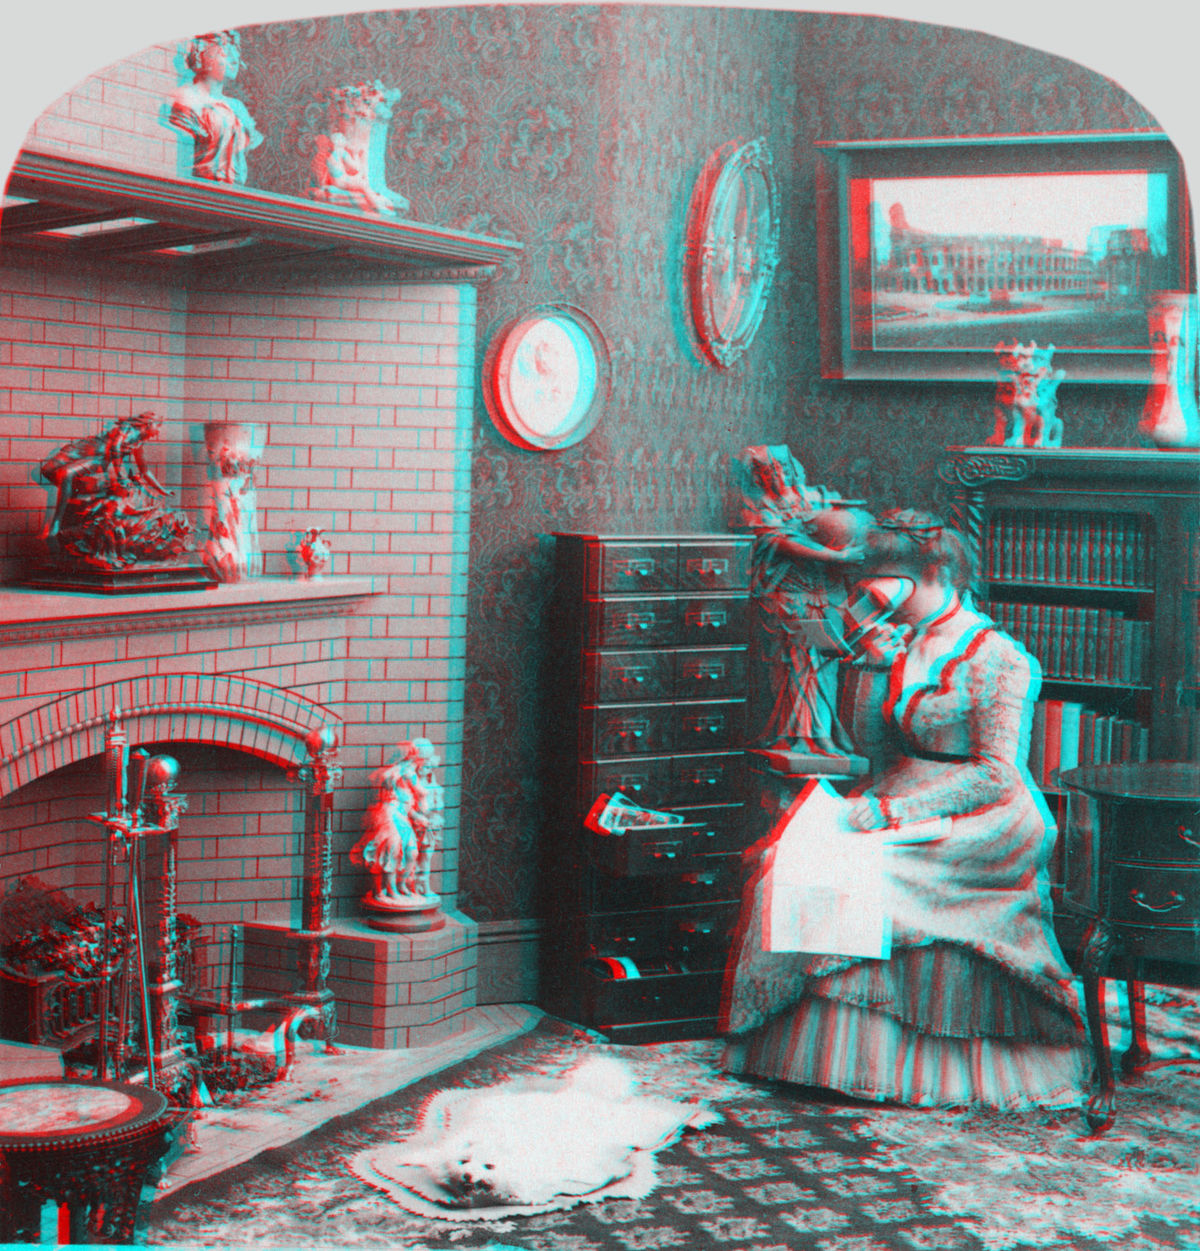
\includegraphics[width=6.5cm]{anaglif.jpg}
 		\captionsetup{font={up, footnotesize}}
    	\caption{Anaglif \cite{anaglif}.}
 		\label{rys4}
\end{figure}

\subsubsection{Wizualizacja wielopasmowa}
Nowa technika wyświetlania obrazów stereoskopowych, znana również pod tytułem INFITEC (ang. Interference filter technique, technika filtrowania interferencyjnego). Główna idea tej techniki jest podobna do technik anaglifowych: pokazanie dwóch obrazów z różniącą się perspektywą, które są wykonane w różnych kolorach. Jednak do osiągnięcia efektu stereoskopowego za pośrednictwem wizualizacji wielopasmowych jest wykorzystany taki fakt, że widmo światła widzialnego można podzielić na fale o różnej długości używając do tego filtrów optycznych \cite{infitec}.

Światło widzialne jest podzielone na 6 części, po 2 na każdy z podstawowych kolorów: czerwony, zielony oraz niebieski. Poszczególne części przeznaczone są dla jednego oka. W ten sposób lekko różniące się barwy docierają do każdego oka z osobna. Wykorzystując niewystarczającą wrażliwośc mózgu na tak niedużą różnicę, technika wizualizacji welopasmowej stwarza obrazy pełnokolorowe.  

\subsubsection{Porównanie technik stereoskopowych}
\begin{table}[H]
\caption{Porównanie technik stereoskopowych.}
\centering
\footnotesize
\label{tab11}
\begin{tabular}{!{\color{sapphire}\vrule width 1pt}m{0.146\textwidth}!{\color{black}\vrule width 1pt}m{0.146\textwidth}!{\color{black}\vrule width 1pt}m{0.146\textwidth}!{\color{black}\vrule width 1pt}m{0.146\textwidth}!{\color{black}\vrule width 1pt}m{0.146\textwidth}!{\color{black}\vrule width 1pt}m{0.146\textwidth}!{\color{sapphire}\vrule width 1pt}}
	\arrayrulecolor{sapphire}\hline
	\Centering\bfseries Nazwa technologii &
	\Centering\bfseries Kolory &
	\Centering\bfseries Rozdzielczość &
	\Centering\bfseries Specjalny monitor &
	\Centering\bfseries Liczba widzów &
	\Centering\bfseries Koszt \\
	\hline
	\arrayrulecolor{black}
	Side by side & Obraz pełnokolorowy & Wysoka & Niekonieczny & Ograniczona & Średni \\ 
	\hline
	Single image & Całkowity brak kolorów & Średnia & Nie & Ograniczona & Niski \\ 
	\hline
	Stereoskopia pasywna & Obraz pełnokolorowy & Wysoka & Tak & Duża & Średni \\ 
	\hline
	Stereoskopia aktywna & Obraz pełnokolorowy & Wysoka & Tak & Ograniczona & Wysoki \\ 
	\hline
	Anaglify & Całkowity brak kolorów & Średnia & Nie & Duża & Bardzo niski \\ 
	\hline
	Wizualizacje wielopasmowe & Obraz pełnokolorowy & Wysoka & Nie & Ograniczona & Bardzo wysoki \\ 
	\arrayrulecolor{sapphire}\hline
\end{tabular}
\end{table}

Po porównaniu opisanych technik stereoskopowych zostały wybrane 2 do głędszego przestudiowania: technika typu syde by side oraz stereoskopia aktywna. 

\newpage
\subsection{Biblioteka OpenGL}
OpenGL (ang. Open Graphics Library, otwarta biblioteka graficzna) jest potężnym systemem graficznym stanowiącym niejako pomost między programistą a sprzętem komputerowym. Procedury OpenGL umożliwiają renderowanie obiektów o rożnych poziomach skomplikowania zaczynając od prostego punktu geometrycznego, linii lub wypełnionego wielokąta do utworzenia najbardziej złożonej, zakrzywionej powierzchni, oświetlonej i odwzorowanej teksturą. OpenGL pozwala programistom na dostęp do prymitywów geometrycznych i obrazowych, przekształcenia modelu, oświetlenia i teksturowania, antyaliasingu i wielu innych funkcji. 

OpenGL obsługuje aplikacje wizualizacji z obrazami 2D traktowanymi jako typy prymitywów, którymi można manipulować podobnie jak obiektami geometrycznymi 3D. Mimo że specyfikacja biblioteki definiuje konkretny potok przetwarzania graficznego, dostawcy platformy mają swobodę dostosowywania konkretnej implementacji OpenGL, żeby osiągnąć sprecyzowane cele w zakresie kosztów i wydajności. Pojedyńcze wywołania mogą być wykonywane na dedykowanym sprzęcie, uruchamiane jako procedury programowe w standardowym systemie CPU (ang. Central Processing Unit, procesor) lub implementowane jako kombinacja zarówno specjalnych procedur sprzętowych, jak i programowych. Taka elastyczność implementacji skutkuje przyśpieszeniem renderowania, w dodatku jest powszechnie dostępna na wszystkich jednostkach od komputerów o niskich kosztach, po wysokiej klasy stacjach roboczych i superkomputerach \cite{openglofficial}.
\subsubsection{Potok przetwarzania}
\begin{figure}[H]
		\centering
 		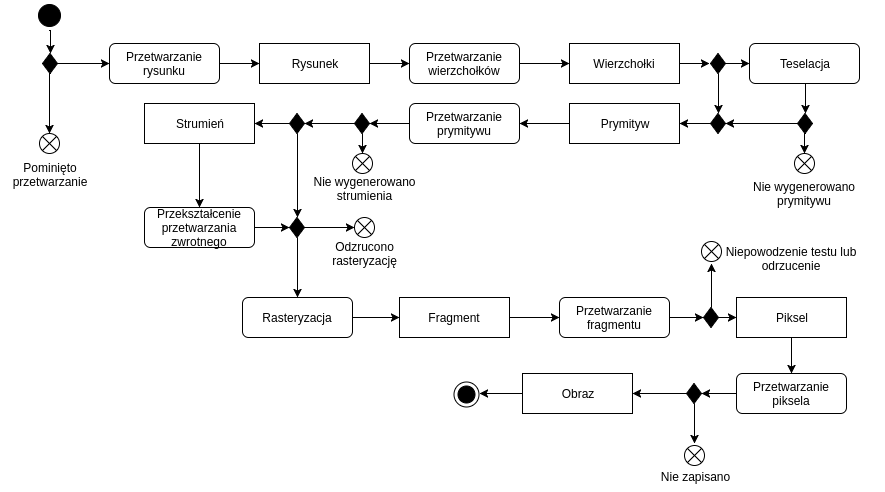
\includegraphics[width=15.5cm]{OpenGL.png}
 		\captionsetup{font={up, footnotesize}}
    	\caption{Schemat potoku przetwarzania.}
 		\label{rys7}
\end{figure}
W OpenGL wszystko jest przedstawione w przestrzeni trójwymiarowej, ale na ekranie obraz widzimy jako listę pikseli 2D, w związku z tym duża część pracy OpenGL polega na zmianie współrzędnych 3D na piksele 2D, które by pasowały do ekranu. Cały proces transformacji jest zarządzany poprzez potok graficzny OpenGL. Taki ciąg jest podzielony na poszczególne kroki, gdzie na wejściu są wymagane dane wyjściowe poprzedniego kroku. Każda z operacji jest dobrze sprecyzowana, gdyż mają one konkretną funkcję. Większość współczesnych kart graficznych posiada setki, czasmi tysiące, małych jąder procesowych do szybkiego przetwarzania danych wejściowych.

\subsubsection{Moduły cieniujące}
Poprzez zgrupowanie poszczególnych kroków w potoku przetwarzania OpenGL powstaje schemat uproszczony. Został on przedstawiony na rys. \ref{rys8}.
\begin{figure}[H]
		\centering
 		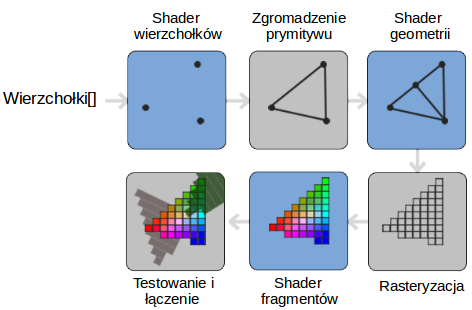
\includegraphics[width=11cm]{pipeline.png}
 		\captionsetup{font={up, footnotesize}}
    	\caption{Skrócony schemat potoku przetwarzania \cite{opengltutorial}.}
 		\label{rys8}
\end{figure}
 
 Dla każdego kroku przetwarzania, w celu przyśpieszenia obliczeń, są uruchamiane nieduże programy w procesorze graficznym --- moduły cieniujące.
 
Te programy są pisane w języku w dużym stopniu podobnym do C --- GLSL (ang. OpenGL Shading Language, język cieniowania OpenGL). GLSL jest dostosowany do wykorzystania w grafice, ponieważ zawiera przydatne funkcje skierowane na manipulacje wektorami i macierzami. Moduły cieniujące zawsze zaczynają się od deklaracji wersji, następnie deklarowane są listy zmiennych wejściowych i wyjściowych, uniformy oraz ich główne funkcje. 

Uniform --- sposób przekazywania danych z aplikacji do procesora i z procesora do modułów cieniujących. Uniformy to zmienne globalne. Skutkuje to tym, że uniform jest unikalny dla każdego obiektu modułu cieniującego i jest osiągalny z dowolnego modułu w każdej chwili jego działania. Ponadto, bez względu na ustawioną wartość uniformy jej nie zmieniają, dopóki nie zostaną zresetowane lub zaktualizowane.
\begin{itemize} 
\itemi Moduł cieniujący wierzchołków (ang. vertex shader). Jest programem, który realizuje pierwszy i zarazem fundamentalny etap potoku ---przetwarzanie danych związanych z wierzchołkami, w tym różnych atrybutów przekazanych wraz z położeniem wierzchołka \cite{slownik}.
\itemi Zgromadzenie prymitywu (ang. primitive assembly). Jest to krok, który za dane wejściowe przyjmuje wszystkie wierzchołki (lub jeden, jeśli wybrana jest flaga GL\_POINTS ) z modułu cieniującego wierzchołków. Na tym etapie przetwarzania są kształtowane prymitywy --- wszystkie wierzchołki są grupowane do zadanego kształtu \cite{opengltutorial}.
\itemi Moduł cieniujący geometrii (ang. geometry shader). Program przyjmuje jako argumenty wejściowe kolekcję wierzchołków, które tworzą zadany kształt. W tym module również istenieje możliwość generowania innych kształtów poprzez emitowanie nowych wierzchołków tworząc nowe (lub inne) prymitywy \cite{slownik}. 
\itemi Rasteryzacja. W tym kroku uzyskane wcześniej prymitywy są mapowane na odpowiadające im piksele na ekranie. W wyniku powstają fragmenty do przetwarzania w kolejnym kroku, lecz zanim zostanie uruchomiony moduł cieniujący fragmentów, jest wykonywane przycinanie. Przyciannie pozwala odrzucić wszystkie fragmenty, które są poza zasięgiem obserwatora. Ów krok pozwala znacznie zwiększyć wydajność całego potoku. Fragment w OpenGL zawiera wszystkie niezbędne dane do wyświetlenia pojedyńczego piksela \cite{slownik}.
\itemi Moduł cieniujący fragmentów. Głównym celem tego programu jest obliczenie końcowego koloru piksela i jest to zazwyczaj etap, na którym występują wszystkie zaawansowane efekty OpenGL. Z reguły moduł posiada wszystkie dane o scenie 3D (takie jak światła, cienie, kolor światła itp.), które są niezbędne dla określenia ostatecznej wartości koloru piksela \cite{slownik}.
\end{itemize}

\newpage
\subsection{Formaty plików 3D}
W celu ponownego wykorzystania skonstruowanych modeli 3D i przesłania ich na różne platformy, tworzone są pliki graficzne. Jednak powstało wiele różnych formatów plików dla różnych aplikacji. Obecnie w grafice komputerowej istnieje ponad 70 odmiennych formatów \cite{formatslist}. Są one wykorzystywane w różnych dziedzinach zaczynając od druku 3D, gier komputerowych, aż po medycynę i nauki przyrodnicze. 

Podstawowym celem formatu pliku 3D jest przechowywanie informacji o modelu w postaci tekstu lub danych binarnych. W szczególności musi on zawierać dane o geometrii modelu, jego wyglądzie, scenie oraz animacjach. Geometria modelu opisuje jego dokładny kształt, do wyglądu zalicza się kolory, tekstury, typy wykorzystanych materiałów. Dane o scenie opisują między innymi położenie światła, kamery i obiektów pereferyjnych. 

U podstaw każdego opragramowania graficznego znajduje się biblioteka niskiego poziomu, taka jak OpenGL czy Direct3D. Biblioteki niskiego poziomu faktycznie rysują modele 3D na ekranie. Modele mogą być również przechowywane i przesyłane jako pliki graficzne. Narzędzia autorskie wspierają modelowanie, zapewniają użytkownikom wygodne metody tworzenia, przeglądania, modyfikowania i zapisywania stworzonych modeli. Często opragamowanie autorskie zawiera w sobie również przeglądarkę 3D --- narzędzie graficzne, które odczytuje, analizuje i transformuje pliki 3D do wewnętrznych formatów, a następnie wyświetla użytkownikowi. Przeglądarki grafiki 3D, narzędzia do tworzenia i transformatory formatów mogą uzyskiwać bezpośredni dostęp do plików 3D lub przechodzić przez funkcje bibliotek narzędzi programowania \cite{formatsinfo}. Opisane relacje są zilustrowane na rys. \ref{rys5}.
\begin{figure}[H]
		\centering
 		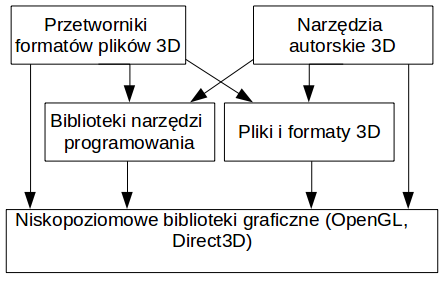
\includegraphics[width=7.0cm]{relacje.png}
 		\captionsetup{font={up, footnotesize}}
    	\caption{Relacje w narzędziach 3D.}
 		\label{rys5}
\end{figure}
Poniżej są przedstawione krótkie opisy najczęściej używanych formatów plików 3D.

\subsubsection{Collada}
Collada to format pliku 3D z rozszerzeniem .DAE, powszechnie jest używany do modelowania w grach komputerowych i filmografii. W całości opiera się na strukturalizowaną reprezentację w XML. Przechowuje wszystkie dane dotyczące modelu 3D, jeden z niewielu formatów wspierających kinematykę i informacje o cieniowaniu.

Struktura formatu zaczyna się w korzeniu zwanym COLLADA, który zawiera elementy mianowane bibliotekami i sceną. Element scena mieści w sobie odnośnik do rzeczywistego początku hierarchii sceny. Natomiast każdy element "biblioteka"\ składa się ze specjalnych zestawów danych dokładnie opisujących model: informacje o siatce (library\_geometries), obrazie (library\_images) itd. Taki podział jest bardzo wygodny pod względem odwoływania się do konkretnych sekcji.  

\subsubsection{STL}
STL (ang. STereoLithography, stereolitografia) jest jednym z najważniejszych formatów plików w dziedzinie druku 3D, tworzenia prototypów oraz komputerowo wspieranej produkcji. Rozszerzenie odpowiadające temu formatowi to .STL. Są dostępne oba rodzaje reprezentacji: tekstowy i binarny, przy czym binarny jest bardziej wykorzystywany ze względu na porównywalnie mały rozmiar plików. 

W STL są pominięte takie dane jak wygląd, scena czy animacje. Jedyne ważne informacje w tym formacie to geometria obiektów, która jest zapisywana w postaci przybliżonej siatki trójkątów. Dla każdego trójkąta są przechowywane 2 rodzaje danych:
\begin{itemize}
\itemi współrzędne wierzchołków;
\itemi współrzędne normalnej, przy tym wektor powinien wskazywać na zewnątrz w odniesieniu do modelu 3D.
\end{itemize}
\begin{figure}[H]
		\centering
 		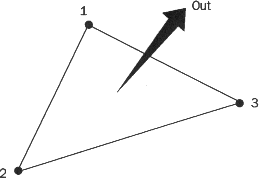
\includegraphics[width=5.0cm]{vertices-and-normal.png}
 		\captionsetup{font={up, footnotesize}}
    	\caption{Wierzchołki i normalna \cite{stlinfo}.}
 		\label{rys6}
\end{figure}
 Dotychczas jest to najprostszy i najbardziej ścisły format przechowywania informacji o modelu 3D. Wadą STL możnaby nazwać brak przechowywania danych o kolorach, ze względu na dynamiczny rozwój technologii druku pełnokolorowego \cite{stlinfo}.

\subsubsection{OBJ}
OBJ jest jednym z najbardziej znanych i wykorzystywanych formatów plików 3D, obecnie nabiera szczególnej wagi w druku 3D. Ten format przechowuje informacje o modelu w postaci tekstu ASCII (rozszerzenie .OBJ) bądź pliku binarnego (rozszerzenie .MOD) \cite{objinfo}.
Format binarny jest zastrzeżony i nieudokumentowany, dlatego poniżej zostanie opisana tylko postać tekstowa formatu. 

OBJ wspiera dane o prostych, wielokątach, krzywych oraz powierzniach o różnych kształtach. Proste i wielokąty są opisywane poprzez wierzchołki, z których się składają. W przypadku krzywych oraz płaszczyzn kluczowymi są punkty kontrolne i inne niezbędne do opisu informacje, w zależności od typu krzywej. Ten format pliku 3D przybliża bądź oblicza doskładną siatkę bez drastycznego zwiększania rozmiaru pliku. Staje się to możliwe dzięki wykorzystaniu krzywych Beziera oraz metody NURBS (ang. Non-Uniform Rational Bezier Spline). 

Format OBJ umożliwia również przechowywanie informacji o kolorach oraz teksturach modelu w towarzyszącym formacie MTL (ang. Material Template Library, Biblioteka Szablonów Materiałów). Plik .OBJ, po sparowaniu z odpowiednim plikiem .MTL, tworzy realistyczny wielokolorowy teksturowany model. Plik MTL jest zapisywany w postaci tekstu ASCII definiującego właściwości materiałów, odbijania światła itd. Dodatkowo MTL wspiera mapy tekstur, w tym przypadku każdy wierzchołek siatki modelu 3D jest przyporządkowywany do dwuwymiarowego obrazu. 

\subsubsection{3DS}
3DS --- to binarny format pliku początkowo wykorzystywany tylko w programie Autodesk 3D Studio. Plik binarny jest oparty o hierarchiczną strukturę "klocków"\ (ang. chunks), w której każdy fragment danych jest umieszczony w bloku z odpowiednim identyfikatorem. Pozwala to analizatorowi składni pominąć fragmenty, które nie są rozpoznawalne, oraz zapewnia możliwość rozszerzenia formatu \cite{3dsformat}. 

3DS przechowuje tylko podstawowe informacje o geomertii, wyglądzie (kolory, tekstury i materiały), scenie oraz animacji. Gromadząc dane o scenie zapisuje położenie kamer i świateł, z wyjątkiem informacji o kierunkowych źródłach światła. Do przybliżenia kształtu obiektu w formacie 3DS używa się siatki trójkątów, ale liczba wierzchołków i wielokątów nie może przekraczać 65536($2^{16}$). 3DS jest obsługiwany praktycznie przez wszystkie pakiety oprogramowania 3D. Ze względu na to, że jednak ten format zbiera tylko podstawowe informacje o modelu 3D, może on być uzupełniony o format MAX (obecnie zastąpiony formatem PRJ), który zawiera dodatkowe informacje specyficzne dla Autodesk 3DS Max, aby umożliwić całkowite zapisanie i załadowanie sceny.

\subsubsection{X3D}
Początkowo X3D nazywał się VRML (rozszerzenie pliku .WRL), z ang. Virtual Reality Modeling Language, czyli Język Modelowania Rzeczywistości Wirtualnej. Format został opracowany na potrzeby WWW (ang. World Wide Web), z czasem został zastąpiony przez X3D. Jest oparty o składnię XML.

X3D wykorzystuje siatkę wielokątów do zakodowania kształtu modelu, umożliwia przechowywanie wyglądu i danych, które wiążą się z tym parametrem. Na przeciągu ostatnich lat rozwoju tego formatu zostały dodane: kodowanie NURBS powierzchni geometrii a także możliwość gromadzenia danych o scenie i animacjach.

\subsubsection{Porównanie formatów plików}
Poniższa tabela przedstawia porównanie opisanych formatów plików 3D pod względem różnorodności przechowywanych danych. 
\begin{savenotes}
\begin{table}[H]
\caption{Macierz funkcjonalności najpopularniejszych formatów plików 3D}
\centering
\footnotesize
\label{tab1}
  \begin{tabular}{!{\color{sapphire}\vrule width 1pt}c!{\color{black}\vrule width 1pt}c!{\color{black}\vrule width 1pt}c!{\color{black}\vrule width 1pt}c!{\color{black}\vrule width 1pt}c!{\color{black}\vrule width 1pt}c!{\color{black}\vrule width 1pt}c!{\color{black}\vrule width 1pt}c!{\color{black}\vrule width 1pt}c!{\color{black}\vrule width 1pt}c!{\color{black}\vrule width 1pt}c!{\color{sapphire}\vrule width 1pt}}
	\arrayrulecolor{sapphire}\hline
    \multirow{2}{*}{\bfseries Format} &
      \multicolumn{3}{c!{\color{black}\vrule width 1pt}}{\bfseries Geometria} &
      \multicolumn{3}{c!{\color{black}\vrule width 1pt}}{\bfseries Wygląd} &
      \multicolumn{3}{c!{\color{black}\vrule width 1pt}}{\bfseries Scena} &
     \multirow{2}{*}{\bfseries Animacje}\\
     \cline{2-10}
    & Przybl.\footnote{Przybliżona siatka}&Dokł.\footnote{Dokładna siatka}&CSG\footnote{CSG (ang. constructive solid geometry, strukturalna geometria bryły) – technika definiowania nowych brył poprzez łączenie innych brył}& Kolor& Materiał&Tekstura&Kamera&Światło&Pozycje& \\
    \hline
    Collada & X & X &  & X & X & X & X & X & X & X\\   
    \arrayrulecolor{black}
	\hline
    STL & X &  &  &  &  &  &  &  &  & \\
    \hline
    OBJ & X & X &  & X & X & X &  &  &  & \\
    \hline
    3DS & X &  &  & X & X & X & X & X & X & \\ 
    \hline
    X3D & X & X & X & X & X & X & X & X & X & X\\     
   \arrayrulecolor{sapphire}\hline
  \end{tabular}
\end{table}
\end{savenotes}
Z tabeli wynika, że najwięcej informacji przechowują formaty Collada i X3D. W niszej pracy dyplomowej zostanie wykorzystany format Collada, ze względu na strukturę oraz możliwość łatwego użycia z poziomu kodu źródłowego programu.

\newpage
\subsection{Biblioteki do czytania i pisania modeli 3D}
Niestety, graficzne biblioteki niskiego poziomu takie jak OpenGL czy DirectX nie zapewnią żadnego mechanizmu do ładowania, zapisywania lub manipulowania modelami 3D. Dlatego, powstała potrzeba stworzenia nowych bibliotek ułatwiających te czynności. 
\subsubsection{Assimp}
Assimp (ang. Open Asset Import Library, Biblioteka Importowania Zasobów) to przenośna biblioteka do importowania różnych dobrze znanych formatów modeli 3D w jednolity sposób. Najnowsza wersja potrafi nie tylko czytać, ale również i zapisywać pliki 3D i dlatego nadaje się jako transformator modeli 3D do ogólnego zastosowania. Assimp jest napisana w języku C ++, istnieje również API (ang. Application Programming Interface, Interfejs Programistyczny Aplikacji) w języku C, a także jest powiązana z innymi językami programowania, w tym C \#, .net, Python i D.

Assimp ładuje wszystkie formaty modeli wejściowych do jednej prostej struktury danych w celu dalszego przetwarzania. Podstawowy zestaw funkcji jest rozszerzany przez różne narzędzia do przetwarzania końcowego. Przykładem rozszerzenia mogą posłużyć często potrzebne operacje, takie jak obliczanie wektorów normalnych i stycznych \cite{assimp}.
\subsubsection{Lib3ds}
Lib3ds to darmowa alternatywa dla pakietu 3DS File Toolkit firmy Autodesk do zarządzania plikami 3DS. Ta biblioteka jest w całości napisana w języku C, wspierana przez takie platformy jak GNU, UNIX, Mac OS X, Microsoft Visual C++ 8.0. Jest łatwo integrowalna z biblioteką OpenGL \cite{lib3dsofficial}. 

Celem lib3ds jest uproszczenie tworzenia filtrów do czytania i pisania plików formatu 3DS. Ta biblioteka jest obsługiwana na różnych rodzajach procesorów (big oraz little endian), wspiera moduły wektorowe, kwaterniony, macierze, proste struktury danych, które można łatwo modyfikować, ocenę wszystkich danych animacji. Istnieje możliwość załadowania większości fragmentów 3DS, sekcje: materiały, kamera, światło, siatka i klucze \cite{lib3dsdirectory}.

\newpage
\subsection{ALICE}
ALICE (ang. A Large Ion Collider Experiment, czyli Wielki Eksperyment Zderzacza Jonów) jest jednym z największych na świecie eksperymentów fizycznych. Celem tego eksperymentu jest pomiar zderzeń ciężkich jonów przy najwyższych osiągalnych obecnie energiach przy użyciu detektora na Wielkim Zderzaczu Hadronów w międzynarodowym laboratorium fizyki cząstek CERN w Genewie. 

Detektor ALICE został zaprojektowany tak, aby w jak najbardziej kompletny sposób badać cząstki powstałe w kolizjach, które mają miejsce w środku akceleratora. Do zrealizowania założeń, używa się wielu warstw różnych detektorów, z których każda dostarcza innych informacji o przebiegu zderzenia. Dane są gromadzone w sposób umożliwiający zrekonstruowanie i zbadanie ewolucji systemu cząstek w przestrzeni i czasie \cite{aliceofficial}. 

\subsubsection{Eksperyment}
W ekstremalnych warunkach temperatury i (lub) gęstości materia hadronowa topi się w osoczu wolnych kwarków i gluonów --- tak zwanej plazmy kwarkowo-gluonowej (ang. quark–gluon plasma --- QGP). Aby stworzyć odpowiednie warunki w laboratorium, ciężkie jony (np. cząstki ołowiu) przyśpiesza się do niemal prędkości światła, po czym jest powodowana kolizja. Kluczowym rozważaniem dotyczącym eksperymentu ALICE jest zdolność do badania chromodynamiki kwantowej (ang.  quantum chromodynamics --- QCD) i kwarków w tych ekstremalnych warunkach. Odbywa się to przy użyciu cząstek, utworzonych wewnątrz gorącej objętości podczas jej rozszerzania się i ochładzania. Cząstki te żyją wystarczająco długo, aby dotrzeć do wrażliwych warstw detektora zlokalizowanych wokół obszaru oddziaływania.

 Fizyka w ALICE polega na tym, żeby być w stanie zidentyfikować wszystkie cząstki (tj. określić, czy są to elektrony, fotony, piony itd.), czy też określić ich ładunek. Wiąże się to w większości z różnymi sposobami oddziaływania cząstek z materią \cite{aliceexperiment}.

\subsubsection{Ślady cząstek i detektory}
Zespół detektorów cylindrycznych (od wewnątrz na zewnątrz: ITS\footnote{The Inner Tracking System}  Drift, ITS Strips, TPC\footnote{The ALICE Time Projection Chamber}, TRD\footnote{The ALICE Transition Radiation Detector}) mierzy w wielu punktach (ponad 100 tylko dla TPC) przejście każdej cząstki przenoszącej ładunek elektryczny tak, że trajektoria jest dokładnie znana. Detektory ALICE są osadzone w polu magnetycznym (wytwarzanym przez duży czerwony magnes), wyginając w ten sposób trajektorie cząstek: z krzywizny śladów można znaleźć ich pęd. ITS jest tak precyzyjny, że cząstki, które są generowane przez rozkład innych cząstek o bardzo krótkim czasie życia można zidentyfikować, widząc, że nie pochodzą one z punktu, w którym nastąpiła interakcja ("wierzchołek"\ zdarzenia) \cite{trackingparticles}.

\begin{figure}[H]
		\centering
 		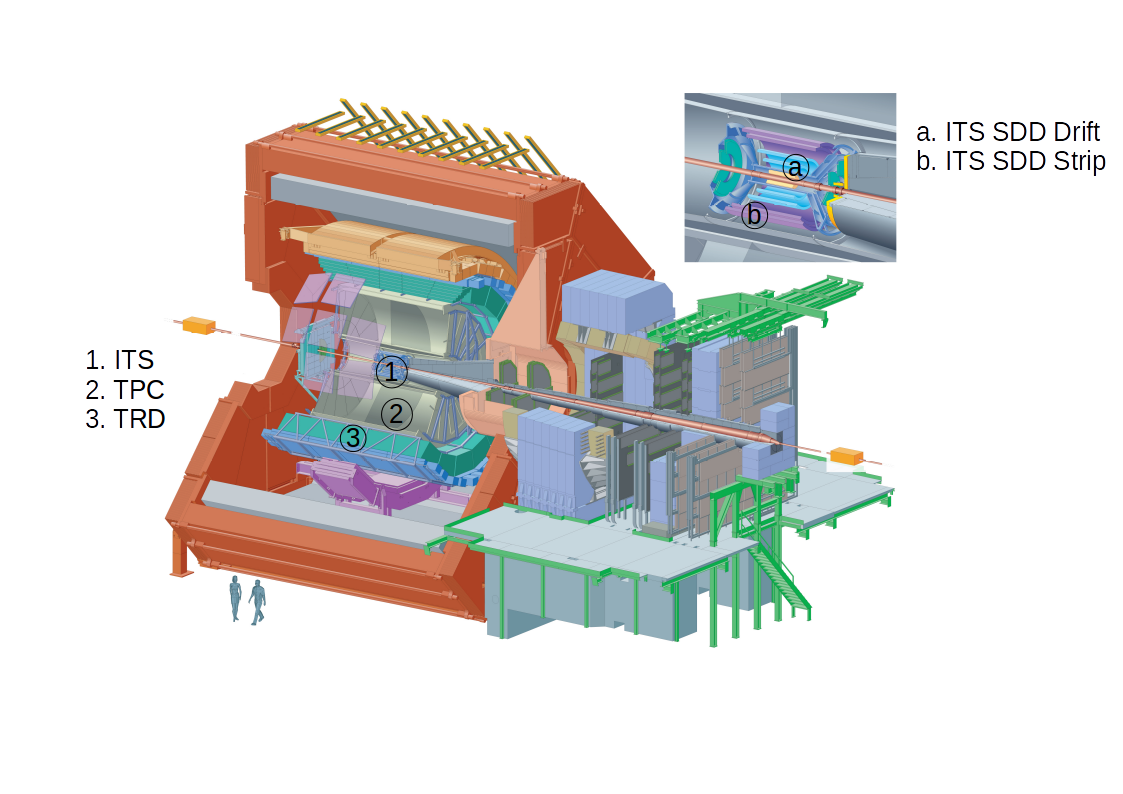
\includegraphics[width=16.0cm]{detector.png}
 		\captionsetup{font={up, footnotesize}}
    	\caption{Detektor ALICE \cite{aliceofficial}.}
 		\label{rys9}
\end{figure}
%\subsubsection{Geometria detektora}
\newpage
\section{Projekt}
\subsection{Wymagania funkcjonalne}
Funkcje jakie musi wykonywać program wraz z opisami są spisane w tabeli \ref{tab2}.
\begin{table}[H]
\caption{Wymagania fukcjonalne.}
\centering
\footnotesize
\label{tab2}
\begin{tabular}{!{\color{sapphire}\vrule width 1pt}m{0.05\textwidth}!{\color{black}\vrule width 1pt}m{0.26\textwidth}!{\color{black}\vrule width 1pt}m{0.50\textwidth}!{\color{black}\vrule width 1pt}m{0.07\textwidth}!{\color{sapphire}\vrule width 1pt}}
	\arrayrulecolor{sapphire}\hline
	\Centering\bfseries Nr &
	\Centering\bfseries Nazwa &
	\Centering\bfseries Opis &
	\Centering\bfseries Priorytet \\
	\hline
	\arrayrulecolor{black}
	1 & Renderowanie torów cząstek & Program wyświetla ślady cząstek, odczytując kształt krzywych z położenia punktów kontrolnych z dostarczonego pliku JSON. & 1 \\ 
	\hline
	1.1 & Poprawne kolorowanie śladów & Tory są poprawnie pokolorowane w zależności od masy cząstek. Dane są pobierane z dostarczonego pliku JSON. & 1 \\
	\hline
	2 & Renderowanie detektora & Program wyświetla detektor ALICE. Geometria detektora jest dostarczona w postaci pliku o rozszerzeniu .dae. Program odczytuje niezbędne dane z pliku, przetwarza je i wyświetla obraz na ekranie. & 1 \\ 
	\hline
	3 & Stworzenie efektu widzenia stereoskopowego & Program umożliwia oglądanie wyrenderowanych obrazów przy pomocy techniki dwóch obrazów obok siebie (ang. side by side). & 1 \\ 
	\hline
	4 & Stworzenie efektu aktywnego widzenia stereoskopowego & Program umożliwia oglądanie wyrenderowanych obrazów przy pomocy techniki aktywnego widzenia stereoskopowego. & 1 \\ 
	\hline
	5 & Możliwość interakcji z użytkownikiem & Program umożliwia użytkownikowi łatwe sterowanie położeniem oraz obrotami kamery. Funkcjonalność jest dostępna zarówno przy oglądaniu zwykłym jak i stereoskopowym. & 2 \\ 
	\arrayrulecolor{sapphire}\hline
\end{tabular}
\end{table}
\subsection{Wymagania niefunkcjonalne}
\begin{table}[H]
\caption{Wymagania niefukcjonalne.}
\centering
\footnotesize
\label{tab3}
\begin{tabular}{!{\color{sapphire}\vrule width 1pt}m{0.05\textwidth}!{\color{black}\vrule width 1pt}m{0.26\textwidth}!{\color{black}\vrule width 1pt}m{0.50\textwidth}!{\color{black}\vrule width 1pt}m{0.07\textwidth}!{\color{sapphire}\vrule width 1pt}}
	\arrayrulecolor{sapphire}\hline
	\Centering\bfseries Nr &
	\Centering\bfseries Nazwa &
	\Centering\bfseries Opis &
	\Centering\bfseries Priorytet \\
	\hline
	\arrayrulecolor{black}
	1 & Przenośność & Program działa bez błędów na różnych systemach operacyjnych (Windows, Linux). W systemie operacyjnym Linux dopuszczalny jest brak funkcjonalności aktywnego widoku stereoskopowego ze względu na zewnętrzne urządzenia. & 1 \\ 
	\hline
	2 & Zrozumiałość & Program jest łatwy w użyciu. & 1 \\ 
	\hline
	3 & Czytelność kodu źródłowego & Kod źródłowy programu jest napisany zgodnie z zasadami, wzorcami i najlepszymi praktykami branży. & 1\\ 
	\hline
	4 & Tolerowanie defektów & Przewidywalne zachowanie programu pomimo pomyłek obsługi lub wprowadzenia błędnych danych. & 1 \\
	\hline
	5 & Przyjazność programu dla użytkownika & Program jest intuicyjny w obsłudze. & 2\\  
	\arrayrulecolor{sapphire}\hline
\end{tabular}
\end{table}
Wskazanie funkcji oprogramowania nie określa wszystkich cech istotnych dla użytkownika \cite{specyfikacja}. Wymagania niefunkcjonalne, które w danym zastosowaniu są ważne, zostały określone i opisane w tabeli \ref{tab3}. Ze względu na badawczą specyfikę niniejszego programu zostały pominięte niektóre zalecane wymagania niefunkcjonalne.

\subsection{Przypadki użycia}
Aktorem w danym kontekście jest użytkownik programu. Przez to, że głównym celem tej oto pracy dyplomowej są wizualizacje, wszystkie przypadki użycia sprowadzają się do oglądania wyrenderowanych scen oraz poruszania się w nich.
\begin{table}[H]
\caption{Przypadki użycia programu}
\centering
\footnotesize
\label{tab4}
\begin{tabular}{!{\color{sapphire}\vrule width 1pt}m{0.05\textwidth}!{\color{black}\vrule width 1pt}m{0.16\textwidth}!{\color{black}\vrule width 1pt}m{0.50\textwidth}!{\color{black}\vrule width 1pt}m{0.17\textwidth}!{\color{sapphire}\vrule width 1pt}}
	\arrayrulecolor{sapphire}\hline
	\Centering\bfseries Nr &
	\Centering\bfseries Nazwa &
	\Centering\bfseries Opis &
	\Centering\bfseries Scenariusz alternatywny \\
	\hline
	\arrayrulecolor{black}
	FU1 & Wyświetlanie torów cząstek & 
	\begin{itemize}
	\itemi Użytkownik uruchamia program.
	\itemi Wybiera opcję zwykłego wyświetlania torów cząstek.
	\itemi Steruje kamerą przy pomocy klawiatury i myszy.
	\end{itemize} & Brak \\ 
	\hline
	FU2 & Wyświetlanie detektora & \begin{itemize}
	\itemi Użytkownik uruchamia program.
	\itemi Wybiera opcję zwykłego wyświetlania detektora.
	\itemi Steruje kamerą przy pomocy klawiatury i myszy.
	\end{itemize} & Brak \\ 
	\hline
	FU3 & Stereoskopowe wyświetlanie obrazów & \begin{itemize}
	\itemi Użytkownik uruchamia program.
	\itemi Wybiera opcję stereoskopowego wyświetlania detektora (lub torów cząstek).
	\itemi Przełącza ekran w tryb 3D oraz zakłada specjalne okulary.
	\itemi Steruje kamerą przy pomocy klawiatury i myszy.
	\end{itemize} & Brak \\ 
	\hline
	FU4 & Aktywne wyświetlanie obrazów stereoskopowych & \begin{itemize}
	\itemi Użytkownik uruchamia program.
	\itemi Wybiera opcję aktywnego wyświetlania obrazu stereoskopowego detektora (lub torów cząstek).
	\itemi Przełącza ekran w tryb aktywnego widzenia 3D oraz zakłada specjalne okulary.
	\itemi Steruje kamerą przy pomocy klawiatury i myszy.
	\end{itemize} & Brak \\ 
	\arrayrulecolor{sapphire}\hline
\end{tabular}
\end{table}
%\subsection{Diagram klas}

\newpage
\subsection{Technologie}
\subsubsection{Dodatkowe biblioteki graficzne}
Biblioteka ładująca OpenGL (ang. OpenGL Loading Library) wciąga wskaźniki do funkcji OpenGL w środowisku wykonawczym, rdzeniu i rozszerzeniach. Jest to wymagane, aby uzyskać dostęp do funkcji OpenGL w wersjach powyżej 1.1 na większości platform. Duża liczba bibliotek ładujących rozszerzenia zastępuje potrzebę włączenia gl.h. Zamiast tego udostępniają własny nagłówek, który musi zostać użyty. Większość bibliotek ładowania używa specjalnego generatora do skonstruowania kodu, który wciąga wskaźniki funkcji i zawarte nagłówki \cite{LoadingLibrary}. 

GLAD --- biblioteka generująca kod do ładowania GL. Za pomocą GLAD można wygenerować nagłówki lub kod źródłowy dla dowolnej wersji OpenGL, od wersji 1.1 do 4.6. Można również dołączyć dowolne rozszerzenia OpenGL.

GLFW --- biblioteka dla OpenGL rozwijana jako opragramowanie otwarte (ang. open source). GLFW zapewnia łatwość w tworzeniu okien i kontekstów, w obsłudze danych i zdarzeń wejściowych. Biblioteka jest napisana w języku C, dzięki czemu jest multiplatformowa.  

Obsługę wielu okien, monitorów, ramp o wysokiej rozdzielczości DPI i gamma wymienia się jako jedną z najwiekszych zalet tej biblioteki. Oprócz tego, poprzez odpytywania obsługiwane są klawiatura, mysz, gamepad, czas oraz okna zdarzeń, co jest bardzo wygodne w zarządzaniu podczas tworzenia wizualicji. W dodatku GLFW ma dostęp do rodzimych obiektów i opcji kompilacji dla specyficznych funkcji platform \cite{glfw}.

GLEW (ang. OpenGL Extension Wrangler Library, biblioteka rozszerzeń OpenGL) --- wieloplatformowa biblioteka w C (lub C ++). GLEW zapewnia wydajne mechanizmy określające, które rozszerzenia OpenGL są obsługiwane na platformie docelowej. Rdzeń OpenGL oraz funkcje rozszerzenia są ujawnione w pojedynczym pliku nagłówkowym. Biblioteka została przetestowana na różnych systemach operacyjnych, w tym Windows, Linux, Mac OS X i Solaris \cite{glew}.

GLM (ang. OpenGL Mathematics, matematyka OpenGL) --- nagłówek do biblioteki matematycznej C++, opracowany dla oprogramowania graficznego opartego na specyfikacjach języka GLSL. GLM udostępnia klasy i funkcje zaprojektowane i zaimplementowane z użyciem tej samej konwencji nazewnictwa jak w GLSL. Biblioteka zapewnia rozszerzone możliwości: przekształcenia macierzy i kwaternionów, pakowanie danych, liczby losowe, szumy itd. GLM doskonale działa z OpenGL, nadaje do oprogramowania renderowania i rasteryzacji, przetwarzania obrazu, symulacji zjawisk fizycznych oraz wszelkich kontekstów rozwojowych, które wymagają prostej i wygodnej biblioteki matematycznej \cite{glm}. 

\subsubsection{Glitter}
Założono, że projekt będzie łatwy w użyciu, lecz czasami instalowanie zależności może być bardzo frustrujące, szczególnie w środowiskach, w których brakuje zarządcy pakietów lub uprawnień administracyjnych, dlatego pierwsze skonfigurowanie programu może być dużym wyzwaniem.
Dla zapewnienia przenośności oraz łatwości użycia opracowywanego programu skorzystano z gotowego prostego zestawu dla OpenGL pt. Glitter.

Glitter kompiluje i statycznie łączy wszystkie niezbędne biblioteki. Robi on to za pośrednictwem jednej zależnośći: cmake, która służy do generowania specyficznych dla platformy plików makefile lub plików projektu. Glitter łączy większość zależności potrzebnych do wdrożenia podstawowego mechanizmu renderującego \cite{glitter}, zawiera biblioteki:
\begin{itemize}
\itemi assimp
\itemi glfw
\itemi glm
\itemi glad
\end{itemize}

\subsubsection{JSONcpp}
JsonCpp --- to biblioteka w języku C++ umożliwiająca manipulowanie wartościami JSON, w tym serializację i deserializację ciągów. Dzięki JsonCpp istenieje możliwość odczytać i zapisać plik formatu JSON, dołączyć komentarze w konwencji C++ do elementu podczas parsowania oraz przerobić plik JSON zachowując oryginalne komentarze \cite{jsoncpp}.

Jednym ze sposobów integracji JsonCpp z projektem jest dołączenie plików z kodem źródłowym (pojedynczego pliku .cpp i dwóch plików .h) do projektu oraz ich kompilacja w taki sam sposób, jak każdy inny plik źródłowy. Zapewnia to spójność flag kompilacji i kompatybilności, rozwiązuje problemy powstające podczas budowania bibliotek współdzielonych lub statycznych. 

\subsubsection{Google Test}
Google Test --- to biblioteka do tworzenia testów jednostkowych w C++, może byc skompikowana na różnych platformach (m.in. Posix, Windows). Testy mogą być uruchamiane pojedynczo lub wszystkie naraz. To sprawia, że proces szukania i naprawiania jest bardzo łatwy i intuicyjny\cite{googleTest}.

Spośród wielu bibliotek do testowania jesdnostkowego została wybrana ta, ponieważ przeciwieństwie do wielu innych bibliotek, struktura testowa Google ma wbudowane asercje. Można je wdrażać do oprogramowania, w którym obsługa wyjątków jest wyłączona (zazwyczaj ze względu na wydajność). Tak więc asercje mogą być również bezpiecznie stosowane w destruktorach \cite{ibmGoogle}.

Przeprowadzanie testów jest proste. Wystarczy nawiązać połączenie z wcześniej zdefiniowanym makrem RUN\_ALL\_TESTS, wtedy gdy w innych bibliotekach musi być stworzona lub wprowadzona oddzielna klasa uruchamiająca wykonanie testu. 
\newpage
\section{Część weryfikacyjna}
\subsection{Macierze modelu, widoku, projekcji}
Obraz wyświetlany na ekranie --- to wierzchołki o konkretnych współrzędnych dwuwymiarowych przedstawiające scenę 3D, lecz początkowo scenę tworzy się w przestrzeni trójwymiarowej. Przejścia z jednego układu współrzędnych na inny są znacznie wygodniejsze przy użyciu macierzy transformacji: modelu, widoku oraz projekcji. 

Lokalny układ współrzędnych to taki układ, w którym obiekt ma swój początek. Położenia wierzchołków obiektu są zmieniane względem początku układu lokalnego. Lokalne układy współrzędnych są przeliczane na współrzędne świata, dzięki temu obiekty są rozmieszczane w różnych miejscach sceny. W kolejnych krokach układ współrzędnych świata jest przekształcany na widok z perspektywy kamery. Po wprowadzeniu współrzędnych do widoku są one zmieniane na współrzędne rzutni. Decydującym faktem jest to, że współrzędne rzutni są przetwarzane w zakresie (-1.0; 1.0), określając jednoznacznie wierchołki, które mają być wyświetlone na ekranie. Ostateczny obraz powstaje po przeliczeniu współrzędnych rzutni na współrzędne ekranu, które są następnie przesyłane do rasteryzatora. Opisane prześcia i transformacje macierzy są zilustrowane na rys.\ref{rys11}.
\begin{figure}[H]
		\centering
 		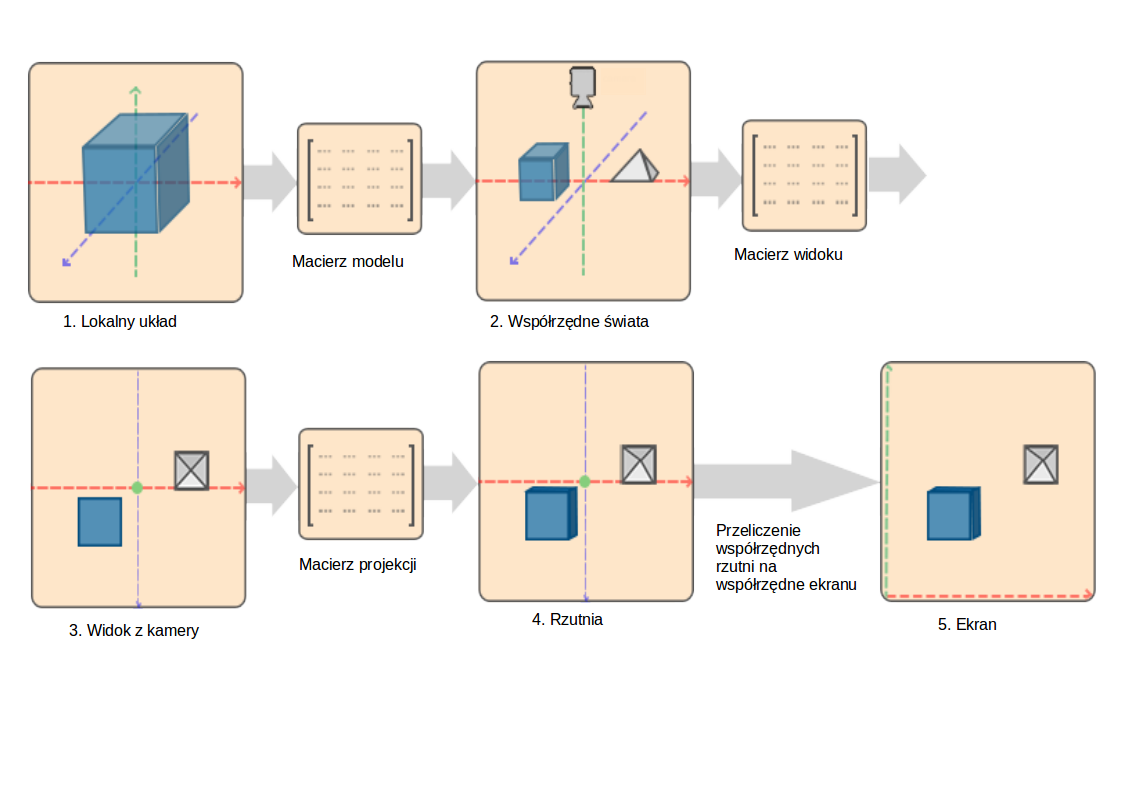
\includegraphics[width=12.0cm]{coordinate_systems.png}
 		\captionsetup{font={up, footnotesize}}
    	\caption{Przejścia z jednego układu współrzędnych na inny \cite{opengltutorial}.}
 		\label{rys11}
\end{figure}
Stąd przyjęto założenie, że wszystkie wierzchołki modelu są w lokalnym układzie współrzędnych obiektu. Natomiast macierz modelu reprezentuje  obiekt w układzie współrzędnych świata, ze względu na możliwość skalowania, obrotu czy translacji. Widok jest z reguły przypisywany do kamery. Macierz projekcji początkowo przypisywana jest do przestrzeni rzutni w zakresie (-1000; 1000) na każdej osi, lecz ostatecznie jest normalizowana do zakresu (-1.0; 1.0). Wszystkie wierzchołki umieszczone poza tym zakresem nie będą widoczne na ekranie.

\subsection{Kamera}
Jednym z wymagań funkcjonalnych było sterowanie kamerą w celu przesunięcia bądź przybliżenia widoku. Umożliwia to plik nagłówkowy Camera.h.

Podchodząc do rozwiązania takiego zadania zakłada się, że za pomocą macierzy widoku wszystkie współrzędne sceny są przekształcane na współrzędne widoku względem położenia i kierunku patrzenia kamery. Stąd do zdefiniowania kamery niezbędne są: 
\begin{itemize}
\itemi położenie kamery w scenie;
\itemi kierunek patrzenia kamery;
\itemi wektora skierowanego w prawo od kamery;
\itemi wektora skierowanego w górę od kamery.
\end{itemize}
W ten sposób został utworzony układ współrzędnych, gdzie położenie kamery jest punktem początkowym, a trzy pozostałe wektory --- to prostopadłe do siebie osie. 

Funkcja glm::LookAt z biblioteki GLM przyjmuje jako argumenty położenie kamery, kierunek patrzenia oraz wektor skierowany w górę (tworzy z tego wektor skierowany w prawo od kamery), zwracając przy tym gotową macierz widoku. W głównym pliku programu została zdefiniowana funkcja processInput, która używając biblioteki GLFW zarządza danymi przychodzącymi z klawiatury. Dzięki tej funkcji łączone są określone klawisze z odpowiednimi zmianami położenia kamery.

Obroty kamery zostały zrealizowane przy użyciu macierzy obrotu i funkcji trygonometrycznych. Wartości odchylenia i nachylenia kamery są pozyskiwane z ruchu myszy, gdzie poziomy ruch myszy wpływa na odchylenie, a pionowy odpowiednio na nachylenie. Zapamiętywana jest pozycja myszy w ostatniej klatce, a w aktualnej jest obliczana różnica wartości aktualnych i zapamiętanych. W zależności od wielkości obliczonych wartośći porusza się kamera. Dla uniknięcia zbyt szybkich albo dużych odchyleń (lub nachyleń) zostały wprowadzone ograniczniki, zmniejszające zakres poruszania kamerą \cite{learnopengl}. 

Również wprowadzono do programu obsługę przybliżenia. Rozwiązano to używając właściwości "pola widzenia"\ : jak pole widzenia staje się mniejsze, rzutowana przestrzeń sceny zmniejsza się, dając iluzję powiększania. Do sterowania powiększaniem używa się kółka myszki.

\newpage
\subsection{Rysowanie ścieżek cząstek}
W celu narysowania ścieżek cząstek niezbędne są wierzchołki składające się na nie. Zgodnie z założeniem początkowym są one odczytywane z pliku JSON. Współrzędne odczytanych wierzchołków są zapisywane do wspólnej tablicy. Wraz ze ścieżkami są odczytywane masy cząstek, po których zostały ślady. Masa cząstki jest później używana do kolorowania toru.

\subsubsection{Odczytanie danych}
Proces odczytania danych ze specjalnie przygotowanego pliku JSON jest realizowany z użyciem biblioteki JsonCpp. W tabeli \ref{tab6} jest przedstawiony kawałek kodu źródłowego, który deserializuje dane JSON (Json::Reader readerTracks) i zapisuje odczytane wartości do tablicy dwuwymiarowej. Json::Value reprezentuje wartość JSON, zmienna ifs przekazuje ścieżkę do pliku do strumienia wejściowego (ang. ifstream, strumień wejściowy do obsługi plików).
\begin{table}[H]
\caption{Kod źródłowy programu. Odczytanie danych z pliku JSON.}
\label{tab6}
\begin{lstlisting}[frame=single]  % Start your code-block

Json::Value objTracks; 
Json::Reader readerTracks; 
// parsowanie dostarczonego pliku do obiektu typu Value;
readerTracks.parse(ifs,objTracks); 

for (Json::Value::iterator it = objTracks["fTracks"].begin(); 
 it != objTracks["fTracks"].end(); ++it){
  int TrackIndex = it.key().asInt();
  for (int i = 0; i < (*it)["fPolyX"].size(); i++){
   tracks[TrackIndex][i*5] = (*it)["fPolyX"][i].asFloat();
   tracks[TrackIndex][i*5 + 1] = (*it)["fPolyY"][i].asFloat();
   tracks[TrackIndex][i*5 + 2] = (*it)["fPolyZ"][i].asFloat();
   tracks[TrackIndex][i*5 + 3] = (*it)["fMass"].asFloat();
   tracks[TrackIndex][i*5 + 4] = 1.0f;
  }
\end{lstlisting}
\end{table}
Zdefiniowana w ten sposób tablica wierzchołków jest wysyłana na wejście modułu cieniującego wierzchołków dla dalszego przetwarzania. Odbywa się to poprzez zaalokowanie pamięci w procesorze graficznym, skonfigurowanie sposobu interpretowania tej pamięci przez OpenGL oraz określenie sposobu wysyłania danych do karty graficznej. Zatem moduł cieniujący wierzchołków przetwarza tylko taką liczbę punktów, jaka została zdefiniowana w pamięci.

\subsubsection{Inicjalizowanie buforów}
Moduł cieniujący wierzchołków pozwala na określenie dowolnych danych wejściowych w postaci atrybutów wierzchołków. Oznacza to, że poszczególne części danych wejściowych są ręcznie przypisywane do atrybutów wierzchołka. W takim przypadku potrzebne jest określenie, w jaki sposób OpenGL będzie interpretować dane przed renderowaniem. Założono, że:
\begin{itemize}
\itemi dane pozycji są przechowywane jako 32-bitowe (4 bajty) wartości zmiennoprzecinkowe;
\itemi każda pozycja składa się z 5 wartości: 3 współrzędnych położenia i 2 pozycji koloru;
\itemi nie ma pustych miejsc w tablicy, wszystkie wartości są obok siebie;
\itemi pierwsza wartość jest początkiem bufora.
\end{itemize}
Używając funkcji glEnableVertexAttribArray określono w jaki sposób dane wierzchołków będą interpretowane. Przykład implementacji powyższych założeń jest przedstawiony w tabeli \ref{tab7}.
\begin{table}[H]
\caption{Kod źródłowy programu. Przekazanie danych do VAO i VBO.}
\label{tab7}
\begin{lstlisting}[frame=single]  % Start your code-block

 glGenBuffers(1, &VBO[TrackIndex]);
 glGenVertexArrays(1, &VAO[TrackIndex]);
 glBindVertexArray(VAO[TrackIndex]);
 glBindBuffer(GL_ARRAY_BUFFER, VBO[TrackIndex]);
 glBufferData(GL_ARRAY_BUFFER, sizeof(tracks[TrackIndex]), 
  &tracks[TrackIndex], GL_STATIC_DRAW);
 glEnableVertexAttribArray(0);
 glVertexAttribPointer(0, 2, GL_FLOAT, GL_FALSE, 5 * sizeof(float), 0);
 glEnableVertexAttribArray(1);
 glVertexAttribPointer(1, 3, GL_FLOAT, GL_FALSE, 5 * sizeof(float), 
  (void*)(2 * sizeof(float)));
 glBindVertexArray(0);
}
\end{lstlisting}
\end{table}
Obiekt tablicy wierzchołków (ang. VAO --- Vertex Array Object) jest powiązany z obiektem bufora wierzchołków. Stąd wszelkie kolejne wywołania atrybutów wierzchołków będą przechowywane wewnątrz VAO. Ma to tę zaletę, że podczas konfigurowania wskaźników atrybutów wierzchołków wystarczy je wywołać tylko raz. Rysując obiekt można po prostu powiązać odpowiedni VAO, dzięki temu przełączanie pomiędzy różnymi konfiguracjami danych a konfiguracją wierzchołków jest bardzo proste.

Do przechowywania dużej liczby wierzchołków w pamięci GPU (ang. Graphics Processing Unit, procesor graficzny), a także do zarządzania tym zasobem posłużono się buforem wierzchołków obiektów (ang. VBO --- Vertex Buffer Objects). Zaletą tego rozwiązania jest bezpośrednie przesyłanie dużej ilości danych do karty graficznej. Gdy niezbędne dane już są w pamięci karty graficznej, moduł cieniujący wierzchołków ma praktycznie natychmiastowy dostęp do wierzchołków, dzięki czemu działa z wyjątkową szybkością.

\subsubsection{Moduły cieniujące}
Następnie były stworzone macierze transformacji. Zostały one przekazane do modułów cieniujących, tam zdefiniowano je jako uniformy i przemnożono ze współrzędnymi wierzchołków. Moduł cieniujący fragmentów jest dość prosty w tym przypadku, gdyż jedynie określa kolor ścieżki, która została po cząstce. Poniżej są umieszczone moduły cieniujące wierzchołków (tabela \ref{tab8}) oraz geometrii (tabela \ref{tab9}).
\begin{table}[H]
\caption{Kod źródłowy programu. Moduł cieniujący wierzchołków.}
\label{tab8}
\begin{lstlisting}[frame=single]  % Start your code-block

#version 420 core
layout (location = 0) in vec3 aPos;
layout (location = 1) in vec2 aColor;
out VS_OUT {
    vec2 color;
} vs_out;
uniform mat4 transform;
uniform mat4 view;
uniform mat4 projection;
void main(){
 vs_out.color = aColor;
 gl_Position = projection * view * transform * 
           vec4(aPos.x, aPos.y, aPos.z, 1.0); }
\end{lstlisting}
\end{table}
\begin{table}[H]
\caption{Kod źródłowy programu. Moduł cieniujący geometrii.}
\label{tab9}
\begin{lstlisting}[frame=single]  % Start your code-block

#version 420 core
layout (lines_adjacency) in;
layout (line_strip, max_vertices = 4) out;
in VS_OUT {
    vec2 color;
} gs_in[];
out vec2 fColor;
void main(void){
 fColor = gs_in[0].color;
 int i;
 for (i = 0; i < gl_in.length(); i++){
  gl_Position = gl_in[i].gl_Position;
  EmitVertex(); } }
\end{lstlisting}
\end{table}

Moduł cieniujący geometrii w przeciwieństwie do modułu cieniującego wierzchołków, posiada wszystkie dane określające prymityw. Dla każdego prymitywu wejściowego, moduł cieniujący geometrii ma dostęp jak do wszystkich jego wierzchołków tak i do informacji o sąsiedztwie, jeśli takie informacje zostały wcześniej określone. W przypadku opracowywanego programu na wejście modułu cieniującego geometrii zostały podane przylegające do siebie kawałki krzywej (ang. lines adjacency). Na wyjściu tego modułu otrzymano jedną spójną ścieżkę.

Pisanie, kompilowanie i zarządzanie modułami cieniującymi może być dość kłopotliwe, dlatego została zaimplementowana klasa Shader. Odczytuje ona moduły z dysku, kompiluje je, łączy oraz sprawdza błędy. 

\subsubsection{Antyalising}
Podczas tworzenia obrazów tórów napotkano problem zniekształcenia linii --- aliasing. Aliasing jest zjawiskiem związanym z rasteryzacją obiektów. Wszystkie wyświetlane prymitywy składają się z pewnej liczby pikseli, dlatego poszczególne punkty rastra są widoczne na urządzeniu końcowym. Poziom zniekształceń zależy od rozdzielczości ekranu. 

Techniki eliminujące efekt aliasingu, nazywane są antyaliasingiem (lub wygładzaniem krawędzi). Najczęściej polegają one na dodaniu pikseli uzupełniających brzegi figury lub procesie nadpróbkowania. Nadpróbkowanie sprowadza się do przeprowadzenia rasteryzacji w rozdzielczości większej niż docelowa, a następnie odpowiedniego skalowania. Biblioteka OpenGL udostępnia obie techniki antyaliasingu. 

W niniejszej pracy została wykorzystana metoda uzupełniająca. Antyaliasing linii w OpenGL wymaga tylko wywołania funkcji glEnable z parametrem GL\_LINE\_SMOOTH oraz włączenia mechanizmu mieszania kolorów. Domyślnie antyaliasing jest wyłączony. 

%Na każdym z umieszczonych obrazów liczba torów jest inna, jak również widoczne są ścieżki o różnych kolorach (wartość określana z masy cząstki). 
%4 obrazy z różnych plików

\newpage
\subsection{Rysowanie detektora}
1. Wczytaj dane poprzez parsowanie Collady (assimp ma wbudowany parser)
2. Stwórz siatkę i policz kolory
3. Wyświetlaj 2.

1 duży obiekt scena w assimpie, z niego wyciągamy resztę danych. 
Problem z plikiem .dae; mój komp nie wyciąga odbrazu.


\newpage
\subsection{Tworzenie obrazu stereoskopowego w technologii side by side}
Wizualicje stereoskopowe w technice side by side wymagają przygotowanych wcześniej dwóch obrazów z różniącą się perspektywą i umieszczenia tych obrazów obok siebie. Dla wyrenderowania różniących się perspektyw w OpenGL muszą być dopasowane regulacja asymetryczna wraz z widokiem renderowanego obszaru. Obszar widoku jest równoległym rzutem asymetrycznym w kształcie ściętego stożka lub równoważnym przesunięciem obiektywu w fotografii. 

Opisywana technika nie wprowadza pionowej paralaksy i jest powszechnie stosowana w renderowaniu stereoskopowym \cite{openglCookbook}. Do zilustrowania koncepcji dla prawego oka (dla lewego oka są wykonywane analogiczne transformację w lustrzanym odbiciu) wykorzystano rys. \ref{rys10}. Przesunięcie reprezentuje wielkość odchylenia dla regulacji asymetrycznej ściętego stożka.

\begin{figure}[H]
		\centering
 		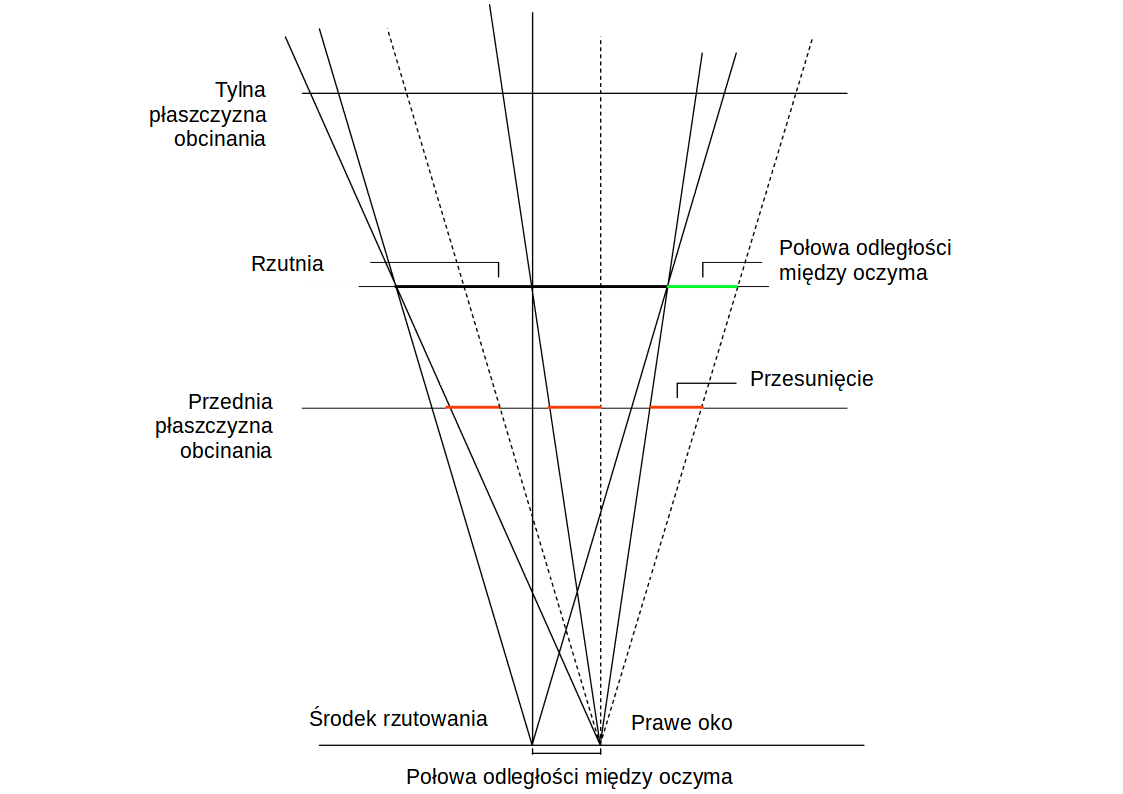
\includegraphics[width=10cm]{stereoscopicGL.png}
 		\captionsetup{font={up, footnotesize}}
    	\caption{Geometria sceny, którą użytkownik widzi z perspektywy prawego oka \cite{openglCookbook}.}
 		\label{rys10}
\end{figure}

Kod źródłowy umieszczony w tabeli \ref{tab5} obrazuje implementację tworzenia rzutowania i wyświetlania macierzy dla stereoskopowej wizualizacji. Kod wykorzystuje odległość między oczyma (zmienna IOD w kodzie), odległość płaszczyzny obrazu (zmienna depthZ) oraz odległość bliskiej płaszczyzny rzutowania (zmienna nearZ).  Wymienione znienne są użyte do określenia wartości przesunięcia. W przedstawionym kodzie źródłowym są zaimplementowane również obliczenie macierzy projekcji i widoku, skorzystano do tego z funkcji biblioteki GLM. 

W tabeli \ref{tab10} zaprezentowano implementację widoku dla każdego oka poprzez odpowiednie ustawienia macierzy projekcji i widoku. Dla każdego oka położenie kamery jest przekładane o połowę odległości między oczyma (jak zostało pokazane na rys. \ref{rys10}). 

Kod źródłowy w tabelach \ref{tab5} i \ref{tab10} był stworzony w oparciu o \cite{openglCookbook}. Ostateczny wynik renderowania składa się z dwóch oddzielnych obrazów po obu stronach ekranu.
\begin{table}[H]
\caption{Kod źródłowy programu. Implementacja przekształceń macierzy stereoskopowych.}
\label{tab5}
\begin{lstlisting}[frame=single]  % Start your code-block

void computeStereoView(float aspect_ratio, float IOD, float depthZ, 
  bool left_eye, glm::vec3 up = glm::vec3(0.0f, 100.0f, 0.0f), 
  glm::vec3 direction_z = glm::vec3(0, 0, 1) ) {
  float left_right_direction = -1.0f;
  if (left_eye)
     left_right_direction = 1.0f;
  double frustumshift = (IOD / 2) * nearZ / depthZ;
  float top = tan(g_initial_fov / 2.0f) * nearZ;
  float right = aspect_ratio * top + frustumshift * left_right_direction;
  float left = -aspect_ratio * top + frustumshift * left_right_direction;
  float bottom = -top;
  g_projection_matrix = glm::frustum(left,right,bottom,top,nearZ,farZ);
  g_view_matrix = glm::lookAt( g_position - direction_z + 
  	glm::vec3(left_right_direction * IOD / 2, 0, 0),
    g_position + glm::vec3(left_right_direction * IOD / 2, 0, 0), up); }
\end{lstlisting}
\end{table}
\begin{table}[H]
\caption{Kod źródłowy programu. Implementacja ustawień macierzy projekcji i widoku.}
\label{tab10}
\begin{lstlisting}[frame=single]  % Start your code-block

void drawStereo (glm::mat4 transform, Shader shader, int trackSize,
     unsigned int VAO[]) {
 glm::mat4 projection = glm::perspective(glm::radians(camera.Zoom),
     (float)SCR_WIDTH / (float)SCR_HEIGHT, 0.1f, 100.0f);
 shader.setMat4("projection", projection);
 glm::mat4 view = camera.GetViewMatrix();
 shader.setMat4("view", view);
 glm::mat4 model = glm::mat4(1.0);
 transform = glm::scale(transform, glm::vec3(0.01, 0.01, 0.01));
 transform = glm::translate(model, glm::vec3(0.0f, 0.0f, -depthZ));
 transform = glm::rotate(model, glm::pi<float>() * rotateY, 
     glm::vec3(0.0f, 1.0f, 0.0f));
 transform = glm::rotate(model, glm::pi<float>() * rotateX, 
     glm::vec3(1.0f, 0.0f, 0.0f));
 GLint transformLoc = glGetUniformLocation(shader.ID, "transform");
 glUniformMatrix4fv(transformLoc, 1, GL_FALSE, glm::value_ptr(transform));
 for (int iterator = 0; iterator < trackSize; iterator++) {
  glBindVertexArray(VAO[iterator]);
  glDrawArrays(GL_LINE_STRIP_ADJACENCY, 0, 4); }}
\end{lstlisting}
\end{table}

\newpage
\subsection{Tworzenie aktywnego obrazu stereoskopowego} 
1) Set the geometry for the view from left human eye 
2) Set the left eye rendering buffers 
3) Render the left eye image 
4) Clear Z-buffer (if the same Z-buffer for left and right image is used) 
5) Set the geometry for the view from right human eye 
6) Set the right eye rendering buffers 
7) Render the right eye image 
8) Swap buffers
\subsection{Weryfikacja poprawności}
\subsubsection{Testy jednostkowe}
Zgodnie z zaleceniami \cite{cleanCode}, testy jednostkowe zostały stworzone dla wszystkich funkcji dostępnych publicznie, w tym funkcji nie zadeklarowanych jako statyczne oraz publicznych konstruktorów i operatorów. Testy obejmują wszystkie główne ścieżki w ramach funkcji i alternatywne gałęzi warunków. Podczas pisania testów jednostkowych trzymano się założenia, że powinny one sprawdzać zarówno przypadki podstawowe, jak i graniczne, dostarczając błędne lub losowe dane, żeby obsługa błędów również została przetestowana.

Główne zasady podczas tworzenia testów jednostkowych:
\begin{itemize}
\itemi jeden test jednostkowy sprawdza tylko jedną rzecz;
\itemi przypadek testowy jest krótki;
\itemi testy przebiegają szybko;
\itemi każdy test działa niezależne, żeby błąd w jednym nie spowodował błędy w innych testach.
\end{itemize}

Głównym celem testów jednostkowych w niniejszej pracy dyplomowej jest sprawdzenie poprawności przekazywania odczytanych danych. Przykładem może posłużyć sprawdzenie czy liczba torów cząstek odczytana z pliku JSON zgadza się z liczbą torów zapisaną do tablicy wierszchołków.

%\subsubsection{Wynik wizualny}

\newpage
\section[Zakończenie]{Zakończenie/Wnioski/Podsumowanie}
%\subsection{na ile zostały spełnione wymagania}
\newpage
\bibliographystyle{plain} % bibliography style
\bibliography{bibliography} % add bibliography
\newpage
\listoffigures
\newpage
\listoftables

\end{document}
